\documentclass[../main.tex]{subfiles}
\usepackage[utf8x]{inputenc}
\usepackage{blindtext}
\usepackage{float}
\usepackage{graphicx}
\usepackage{gensymb}
\usepackage{siunitx}

\begin{document}

Below are views generated for the Moon, Mars, the Didymos asteroid, and the Voyager 1 space probe. Below are the inputs used to generate these views:

\begin{itemize}
    \item \textbf{(Lat, Lon)}:  (38.827778,-77.3), which is the location for George Mason University
    \item \textbf{Start Time}, \textbf{End Time}: 5/1/2022 04:00:00 UTC
    \item \textbf{Minimum Viewing Angle}: \(-90\degree\)
    \item \textbf{Points}: 1
\end{itemize}

The outputs of the commands were then compared with the data available at the Sky Live Online Planetarium (these results were treated as the actual results). Since the azimuth and altitude are manually found on the Sky Live Planetarium view using a mouse, it is hard to gauge the accuracy with certainty, but, the results were within a 10\textsuperscript{th} of a degree of the expected value. 

\section{Moon Results}

\begin{lstlisting}
jweitz@raspberrypi:~/github/ece580_skyfield/src $ python track.py track_planet --planet moon --lat 38.827778 --lon -77.3 --initial_time "2022/05/01-04:00:00" --end_time "2022/05/01-04:00:00" --points 1 --angle -90
Planet: moon
Initial Time: 2022/05/01-04:00:00
End Time: 2022/05/01-04:00:00
(Lat, Lon): (38.827778, -77.3)
Points: 1
Angle: -90
Time: 2022-05-01T04:00:00Z Azimuth: 336.580982 Altitude: -33.263732
\end{lstlisting}

\begin{figure}[H]
    \centering
    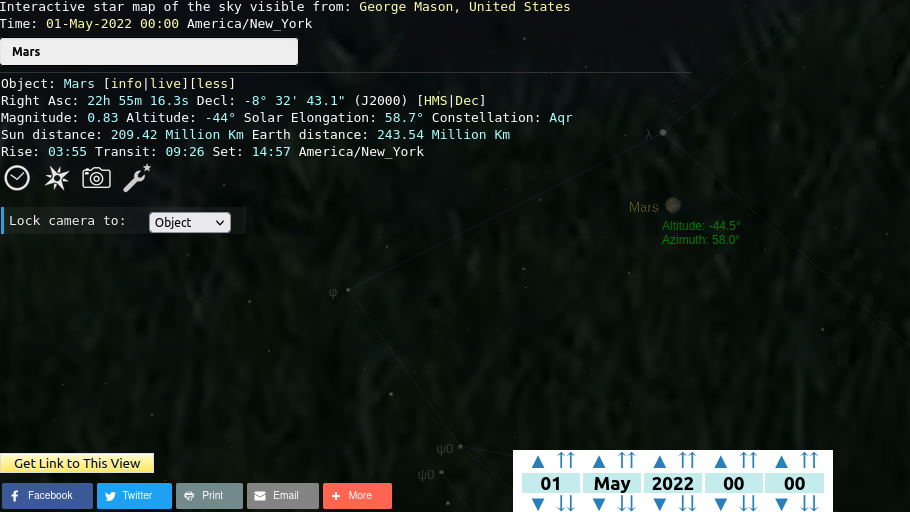
\includegraphics[width=300pt]{components/photos/mars_crop.png}
    \caption{The Sky Live Moon results}
    \label{fig:skylive_moon}
\end{figure}

\section{Mars Results}

\begin{lstlisting}
jweitz@raspberrypi:~/github/ece580_skyfield/src $ python track.py track_planet --planet mars --lat 38.827778 --lon -77.3 --initial_time "2022/05/01-04:00:00" --end_time "2022/05/01-04:00:00" --points 1 --angle -90
Planet: mars
Initial Time: 2022/05/01-04:00:00
End Time: 2022/05/01-04:00:00
(Lat, Lon): (38.827778, -77.3)
Points: 1
Angle: -90
Time: 2022-05-01T04:00:00Z Azimuth: 58.051227 Altitude: -44.587351
\end{lstlisting}

\begin{figure}[H]
    \centering
    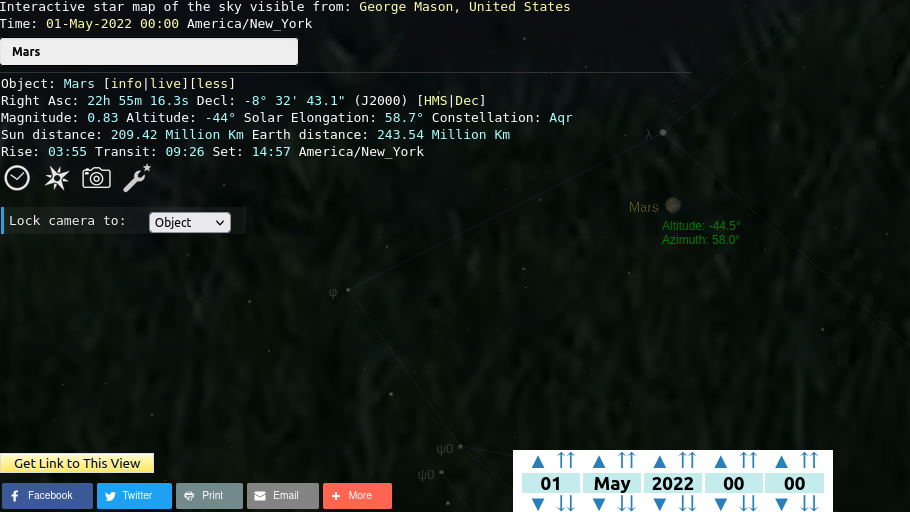
\includegraphics[width=300pt]{components/photos/mars_crop.png}
    \caption{The Sky Live Mars results}
    \label{fig:skylive_mars}
\end{figure}

\section{Didymos Results}

\begin{lstlisting}
jweitz@raspberrypi:~/github/ece580_skyfield/src $ python track.py track_asteroid --lat 38.827778 --lon -77.3 --initial_time "2022/05/01-04:00:00" --end_time "2022/05/01-04:00:00" --points 1 --angle -90                                                                                                                                        
Body: 65803 Didymos
Initial Time: 2022/05/01-04:00:00
End Time: 2022/05/01-04:00:00
(Lat, Lon): (38.827778, -77.3)
Points: 1
Angle: -90
Time: 2022-05-01T04:00:00Z Azimuth: 98.350140 Altitude: -23.373299
\end{lstlisting}

\begin{figure}[H]
    \centering
    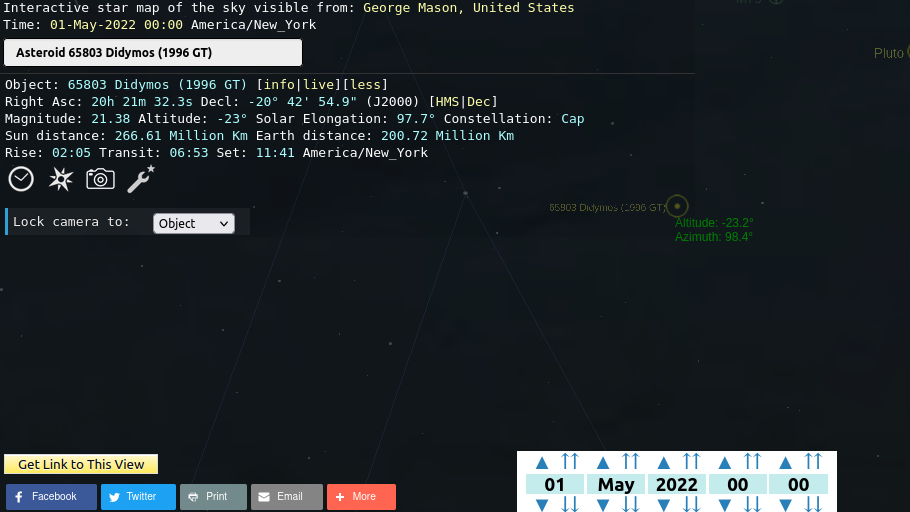
\includegraphics[width=300pt]{components/photos/didymos_crop.png}
    \caption{The Sky Live Didymos results}
    \label{fig:skylive_didymos}
\end{figure}


\section{Voyager 1 Results}

\begin{lstlisting}
jweitz@raspberrypi:~/github/ece580_skyfield/src $ python track.py track_voyager --lat 38.827778 --lon -77.3 --initial_time "2022/05/01-04:00:00" --end_time "2022/05/01-04:00:00" --points 1 --angle -90
Body: Voyager 1
Initial Time: 2022/05/01-04:00:00
End Time: 2022/05/01-04:00:00
(Lat, Lon): (38.827778, -77.3)
Points: 1
Angle: -90
Time: 2022-05-01T04:00:00Z Azimuth: 101.681725 Altitude: 33.507801
\end{lstlisting}

\begin{figure}[H]
    \centering
    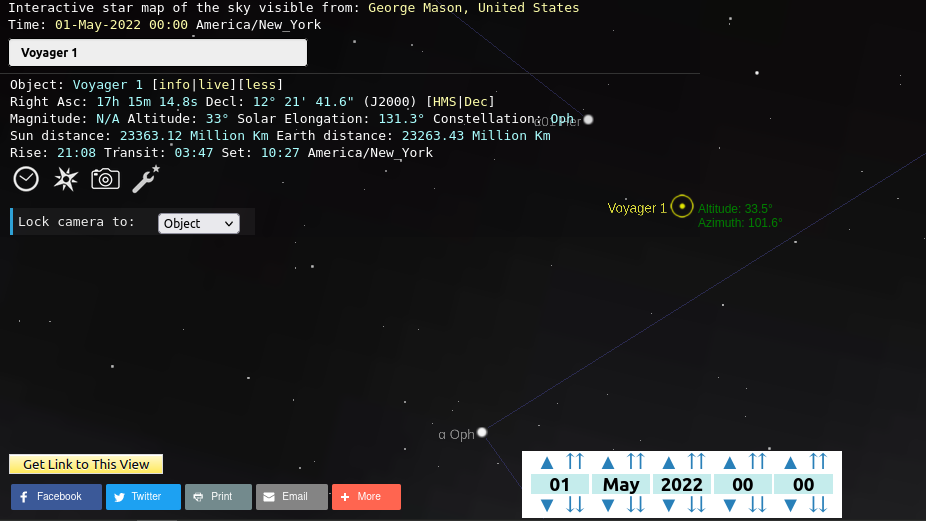
\includegraphics[width=300pt]{components/photos/voyager1_crop.png}
    \caption{The Sky Live Voyager 1 results}
    \label{fig:skylive_voyager}
\end{figure}

\section{Timing and Resource Usage Results}

We bench-marked the library usage on a Raspberry Pi 4B by requesting 1000 views equally spaced in time from 05/01/2022 00:00:00 to 05/02/2022 00:00:00 for Voyager 1 from George Mason University, filtered by \(20\degree\) viewing angle. The results took 4.835 seconds to return, took 100\% of a CPU core while processing, and consumed a maximum of 38.7 MB of memory. We believe that a Raspberry Pi would be perfectly suitable to run this software as an input to an antenna pointing device.

Additionally, we profiled the code to determine the most called functions from the CLI as well as what portions of the code take the longest time to run. The results can be found in Appendix B(\ref{appendix:profile})





\end{document}